% One-round sequence diagram: a re-key round followed by a symmetric-only round.
% Compile: tectonic sequence.tex  (sized for a two-column figure*)
\documentclass[tikz,border=3pt]{standalone}
\usepackage{newtxtext,newtxmath}
\usetikzlibrary{arrows.meta,positioning,calc}

\definecolor{ink}{HTML}{0B0B0B}
\definecolor{ink2}{HTML}{52514E}
\definecolor{rule}{HTML}{B9B8B2}
\definecolor{fillA}{HTML}{F3F2EE}
\definecolor{crypto}{HTML}{E8F1FB}
\definecolor{cryptoedge}{HTML}{2A78D6}
\definecolor{sym}{HTML}{E6F6EF}
\definecolor{symedge}{HTML}{1BAF7A}

\tikzset{
  head/.style={draw=ink2, fill=fillA, rounded corners=2pt, font=\small\bfseries,
               minimum width=3.2cm, minimum height=0.6cm},
  act/.style={draw=rule, fill=white, rounded corners=1.5pt, font=\scriptsize, align=left,
              inner sep=2.5pt, text width=8.0cm},
  msg/.style={-{Stealth[length=2.2mm]}, ink, line width=0.7pt},
  mlbl/.style={font=\scriptsize, fill=white, inner sep=1pt},
  frame/.style={rounded corners=3pt, line width=0.6pt},
  ftag/.style={font=\scriptsize\bfseries, anchor=north west, inner sep=2pt},
}
% Lifeline x positions
\def\xc{0}
\def\xs{15}

\begin{document}
\begin{tikzpicture}[x=1cm, y=1cm]

\node[head] (C) at (\xc, 0) {Client $k$};
\node[head] (S) at (\xs, 0) {Server};
\draw[ink2, densely dashed] (C.south) -- (\xc, -15.1);
\draw[ink2, densely dashed] (S.south) -- (\xs, -15.1);

% ---------- start of round r: broadcast ----------
\draw[msg, ink2] (\xs, -0.9) -- node[mlbl, above] {global weights $w_r$ (plaintext broadcast)} (\xc, -0.9);

% =========================== Re-key round ===========================
\begin{scope}
\fill[crypto!60, frame] (-1.6, -1.35) rectangle (16.6, -10.55);
\draw[cryptoedge, frame] (-1.6, -1.35) rectangle (16.6, -10.55);
\node[ftag, cryptoedge!80!black] at (-1.6, -1.35)
  {Re-key round: $r \bmod N = 0$, \;new epoch $e=\lfloor r/N \rfloor$ \quad(every round in naive PQC)};

\node[act, anchor=north west] at (\xc+0.15, -1.85)
  {$(pk, sk) \leftarrow \mathsf{KEM.KeyGen}()$\\
   $\sigma_C \leftarrow \mathsf{Sign}(sk_C,\ \texttt{init}\,\|\,\mathit{suite}\,\|\,id\,\|\,e\,\|\,pk)$};
\draw[msg] (\xc, -2.95) -- node[mlbl, above] {$\mathsf{HandshakeInit}(id,\ e,\ pk,\ \sigma_C)$} (\xs, -2.95);

\node[act, anchor=north east] at (\xs-0.15, -3.3)
  {check $e = \lfloor r/N \rfloor$ and $e >$ epoch of current session\\
   $\mathsf{Verify}(pk_C, \sigma_C)$ \quad ($pk_C$ pinned at registration)\\
   $(ct, ss) \leftarrow \mathsf{Encaps}(pk)$\\
   $\sigma_S \leftarrow \mathsf{Sign}(sk_S,\ \texttt{resp}\,\|\,\mathit{suite}\,\|\,H(\mathit{init})\,\|\,id\,\|\,e\,\|\,ct)$\\
   $K_e \leftarrow \mathsf{HKDF}(ss,\ \texttt{session}\,\|\,\mathit{suite}\,\|\,id\,\|\,e\,\|\,H(\mathit{init}\,\|\,\mathit{resp}))$};
\draw[msg] (\xs, -5.55) -- node[mlbl, above] {$\mathsf{HandshakeResponse}(id,\ e,\ ct,\ \sigma_S)$} (\xc, -5.55);

\node[act, anchor=north west] at (\xc+0.15, -5.9)
  {$\mathsf{Verify}(pk_S, \sigma_S)$ \quad (blocks MITM re-encapsulation)\\
   $ss \leftarrow \mathsf{Decaps}(sk, ct)$;\quad $K_e \leftarrow \mathsf{HKDF}(ss, \ldots)$ \quad (same info as server)};

\node[act, anchor=north west, fill=fillA] at (\xc+0.15, -7.15)
  {local training from $w_r$ \quad\textit{(excluded from crypto time)}\\
   $k_r \leftarrow \mathsf{HKDF}(K_e,\ \texttt{round}\,\|\,r)$;\quad $\nu \xleftarrow{\$} \{0,1\}^{96}$\\
   $C \leftarrow \mathsf{AES\text{-}GCM}_{k_r}(\nu,\ (n_k, w_k^{r+1}),\ \mathit{AAD}{=}\mathit{mode}\,\|\,id\,\|\,r\,\|\,e)$};
\draw[msg] (\xc, -8.75) -- node[mlbl, above] {$\mathsf{EncryptedUpdate}(id,\ r,\ e,\ \nu,\ C)$} (\xs, -8.75);

\node[act, anchor=north east] at (\xs-0.15, -9.1)
  {reject unless header $r$ = current round, $r >$ last accepted, $e = \lfloor r/N \rfloor$\\
   decrypt with $k_r$ and AAD built from \emph{server} state (header never trusted)\\
   validate, then $\mathsf{FedAvg}$ over accepted updates $\rightarrow w_{r+1}$};
\end{scope}

% =========================== Symmetric-only round ===========================
\draw[msg, ink2] (\xs, -11.0) -- node[mlbl, above] {global weights $w_{r+1}$} (\xc, -11.0);
\begin{scope}
\fill[sym!70, frame] (-1.6, -11.45) rectangle (16.6, -14.9);
\draw[symedge, frame] (-1.6, -11.45) rectangle (16.6, -14.9);
\node[ftag, symedge!70!black] at (-1.6, -11.45)
  {Symmetric-only round $r{+}1$: $(r{+}1) \bmod N \neq 0$, \;same epoch $e$ \quad(amortized and classical)};

\node[act, anchor=north west, fill=fillA] at (\xc+0.15, -11.95)
  {local training from $w_{r+1}$\\
   $k_{r+1} \leftarrow \mathsf{HKDF}(K_e,\ \texttt{round}\,\|\,r{+}1)$;\quad fresh $\nu$\\
   $C \leftarrow \mathsf{AES\text{-}GCM}_{k_{r+1}}(\nu,\ (n_k, w_k^{r+2}),\ \mathit{mode}\,\|\,id\,\|\,r{+}1\,\|\,e)$};
\draw[msg] (\xc, -13.55) -- node[mlbl, above] {$\mathsf{EncryptedUpdate}(id,\ r{+}1,\ e,\ \nu,\ C)$} (\xs, -13.55);
\node[act, anchor=north east] at (\xs-0.15, -13.85)
  {same checks; decrypt; validate; $\mathsf{FedAvg} \rightarrow w_{r+2}$\\
   no KEM and no signature operations; no handshake bytes};
\end{scope}

\end{tikzpicture}
\end{document}
